\section{Particle Accelerators and CERN}

\subsection{Particle Accelerators}

%The first modern particle accelerators started to be conceived at the beginning of the 1900s. Those
%first accelerators, such as the Cockroft-Walton generator, used voltage multipliers to generate
%electric fields in order to accelerate particles.  Voltage multipliers are nowadays still an
%important piece of equipment as they are used in devices requiring high voltage, such as X-Ray
%machines, CRT monitors, microwaves or as part of an accelerator complex.  Those early technologies
%were namely used to perform the first artificial nuclear disintegration.

\todo{GPT}

The history of particle accelerators is a captivating narrative that spans over a century of
scientific innovation and discovery. It is a journey that has fundamentally transformed our
understanding of the universe's fundamental particles and their interactions. The concept of
accelerating particles to high speeds originated in the late 19th century, with early experiments
conducted by pioneers such as J.J. Thomson and Ernest Rutherford, who utilized basic devices like
cathode ray tubes to propel electrons.  One of the earliest breakthroughs in accelerator technology
was the Cockcroft-Walton accelerator, introduced in 1932 by John Cockcroft and Ernest Walton. This
pioneering device employed voltage multipliers to accelerate protons and ions, enabling the first
artificial nuclear disintegration—a milestone that earned them the Nobel Prize in Physics in 1951.
Building upon this achievement, the development of the synchrotron in the 1940s and 1950s by
scientists like Edwin McMillan and Vladimir Veksler marked a significant stride. Synchrotrons
harnessed magnetic fields to bend and accelerate charged particles in circular paths, advancing the
study of particle properties.  A key turning point emerged with the establishment of CERN (the
European Organization for Nuclear Research) in 1954, which culminated in the creation of the Proton
Synchrotron (PS) in 1959. This marked the emergence of a powerful era in accelerator science,
enabling the discovery of novel particles and laying the groundwork for the formulation of the
Standard Model of particle physics. Throughout the 1960s and 1970s, the advent of bubble chambers
and bubble chamber detectors provided researchers with the ability to trace the paths of charged
particles, leading to the revelation of various particles and their intricate interactions.  Yet,
the true marvel of accelerator technology came to the forefront with the construction of the Large
Hadron Collider (LHC) at CERN, which commenced operation in 2008. The LHC, an awe-inspiring
27-kilometer ring of superconducting magnets, propels protons and heavy ions to velocities nearing
the speed of light. The LHC's monumental achievement—the discovery of the Higgs boson in 2012—marked
a crowning moment in particle physics, solidifying the vital role of particle accelerators in
unraveling the fabric of the cosmos.  As particle physicists peer into the future, the quest
continues. Concepts such as linear colliders and advanced circular colliders are on the horizon,
promising to delve even deeper into the enigmatic realm of fundamental particles and the forces that
govern them. The history of particle accelerators underscores the profound human endeavor to explore
the most intricate mysteries of the universe, revealing the intricate dance of particles that shape
the cosmos and expanding the horizons of human knowledge.



\subsection{The CERN Complex}


\todo{GPT}
The CERN complex, located near Geneva, Switzerland, is a prominent center for particle physics
research. Its centerpiece is the Large Hadron Collider (LHC), the world's largest particle
accelerator with a 27-kilometer circumference. Here, protons and heavy ions are accelerated to near
light speed and collide at various points for fundamental particle studies. Surrounding the LHC are
significant particle detectors, including ATLAS, CMS, ALICE, and LHCb, designed to capture and
analyze particles generated during these collisions.  CERN also includes linear accelerators, the
Proton Synchrotron (PS), Super Proton Synchrotron (SPS), and Antiproton Decelerator (AD),
contributing to particle acceleration and antimatter research. Alongside these facilities, CERN
houses the Theoretical Physics Department, where theorists collaborate with experimentalists. With
research, administrative buildings, laboratories, and workshops, CERN provides a comprehensive
environment for scientific exploration. Its history, including the 2012 discovery of the Higgs
boson, underscores its importance in advancing particle physics and highlighting international
scientific cooperation.



% ===============================
%             LHC
% ===============================
\subsection{\todo{The Large Hadron Collider}}

The Large Hadron Collider (LHC), is a circular particle accelerator primarily designed to collide
protons for fundamental particle physics research. It can, occasionally over the year, also collide
ions such as oxygen or lead for specifics studies. At the time of writing, in 2024, it holds several
records, such as being the largest and most powerful accelerator in the world. The LHC is composed
of two beams pipes, being able to accelerate two particle beams from an injection energy of $450$GeV
to an energy of $6,800$GeV, before colliding them in four detectors: ATLAS, CMS, Alice and LCHb.

Well publicized, the LHC is often depicted via its superconducting dipole magnets, housed in a blue
cryostat, aimed at cooling the coils. \cref{fig:3d_cut_dipole} shows a 3D cut of such magnets. The
LHC is in majority composed of those \textit{main} dipoles, as it holds $1,232$ of them, being each
about 14 meters long. Superconducting materials like Niobium-Titanium (NbTi) are utilized, as
conventional materials such as copper would melt under the current strain. There are indeed around
$12,000$ amperes supplied to generate the magnetic fields necessary for bending the trajectory of
the particles.
Those particles travel at nearly the speed of light (more precisely, $99.99999905\%$ of it),
effectively going around the tunnel about $11,200$ times per second.

\begin{figure}[!htb]
    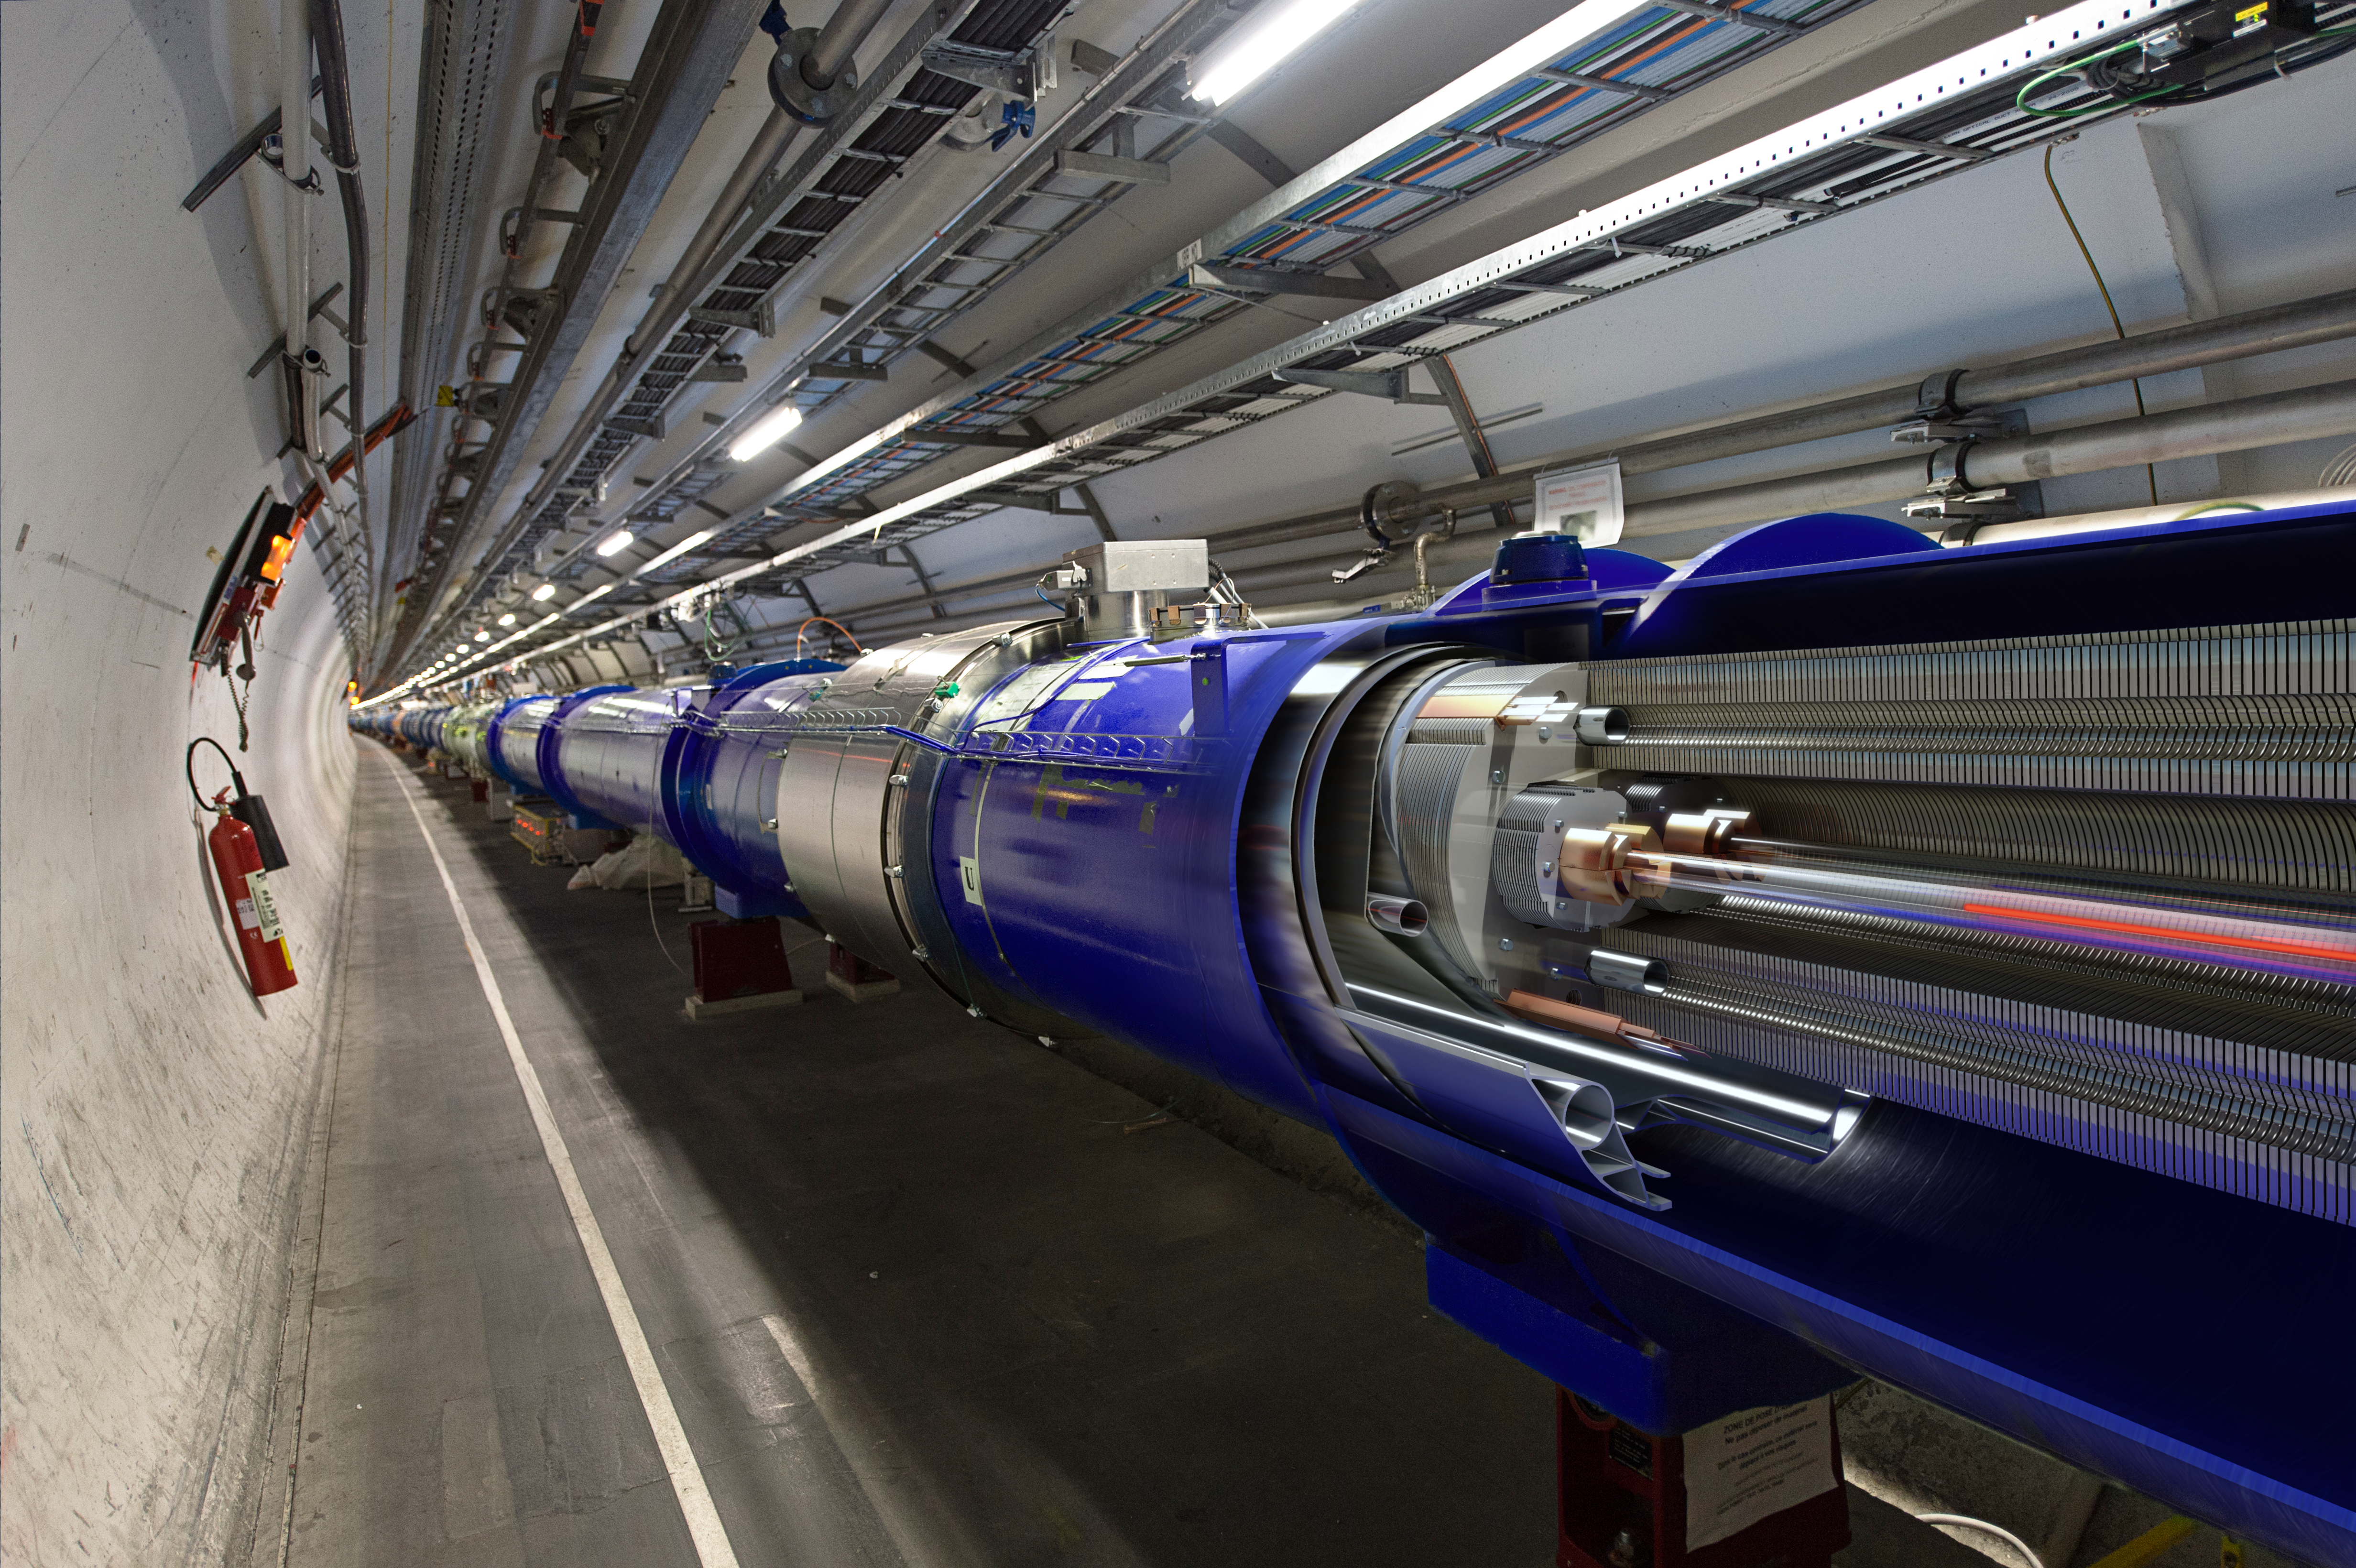
\includegraphics[width=\textwidth]{chapters/01_Introduction/images/lhc_3D_cut.png}
    \caption{3D cut of a main LHC dipole~\cite{noauthor_cern_nodate}. Both beam pipes can be seen
    surrounded by the coils, strongly clamped by the yokes.}
    \label{fig:3d_cut_dipole}
\end{figure}


\paragraph{Straight Sections and Arcs}
The LHC is not a perfect circle. It is indeed composed of four \textit{straight} sections, called
the \textit{Interaction Regions} (IPs) where detectors or instrumentation are placed. Connecting
those sections, the \textit{arcs} are where the majority of the magnets are placed, housing dipoles,
quadrupoles, sextupoles, octupoles and their respective correctors. \cref{fig:introduction:lhc_irs}
shows how the instrumentation, detectors and arcs are distributed along the ring.

\begin{figure}[!htb]
    \centering
    \includegraphics[width=0.5\textwidth]{./images/irs.png}
    \caption{Schematic of the LHC layout.}
    \label{fig:introduction:lhc_irs}
\end{figure}


\paragraph{Arc Cells}

Each arc is made up of 23 cells. Magnets are organized in a standard FoDo structure
(see \ref{section:courant_snyder}), as shows \cref{fig:introduction:lhc_arc_cell}.
\textit{Dipoles} are responsible for bending the trajectory of the particles. Their associated
correctors, the orbit correctors, mitigate any possible drift in path.
\textit{Quadrupoles} are used to control the beam size along the ring. Their effect is focusing in
one plane and defocusing in the other. Their associated correctors control the oscillations of the
beam (see tune, \ref{section:courant_snyder}) and possible field imperfections.
\textit{Sextupoles} correct chromaticity, being a misfocus from quadrupoles due to particles having
a different momentum than the reference particle.
\textit{Octupoles} are used to stabilize the beam by introducing Landau
Damping~\cite{gareyte_landau_1997}. The associated correctors correct higher order chromaticity
effects as well as amplitude dependant tune shifts.
\textit{Decapoles} correctors aim at correcting even a higher chromaticity order.

\begin{figure}[H]
    \centering
    \includegraphics[width=1\textwidth]{./images/lhc_cell.png}
    \caption{Schematic of an LHC Arc cell~\cite{bruning_lhc_2004}.}
    \label{fig:introduction:lhc_arc_cell}
\end{figure}



% ===============================
%          Parameters
\subsubsection{\todo{Parameters}}

optics, pilot bunches

\begin{figure}[H]
    \includegraphics[width=\textwidth]{./images/lhc_cycle.pdf}
    \caption{Simplified illustration of a standard LHC cycle. Courtesy of Félix
    Soubelet~\cite{felix_soubelet_local_2023}} \label{fig:cern_complex:cycle}
\end{figure}


% ===============================
%   Harmonics and Field Errors
\subsubsection{\todo{Harmonics and Field Errors}}

Real-life magnets never have a single field as one would like. Instead, so called 
\textit{allowed harmonics} exist due to the geometry of the coil. As such, the main dipoles of the
LHC can exhibit fields similar to sextupoles, decapoles, decatetrapoles and so
on~\cite{deniau_magnetic_2009}. Manufacturing imperfections also add fields errors outside of the
scope of the allowed ones. Dipoles are indeed found to generate octupolar field errors.

During the design of the LHC, the main dipoles have been identified to generate significant field
errors. Magnetic measurements of those various fields were thus taken and magnetic tables built
based on real-life magnets nowadays installed in the machine. Those magnetic tables, computed for
each LHC configuration by \textit{WISE}~\todo{cite} are used by simulation softwares.
Predictions of field errors and compensating strength for the correctors is computed by the Field
Description for the LHC (\textit{FiDeL}, \cite{noauthor_fidel_2021}). FiDeL is used in the LHC
control system in operation to steer the LHC.

%\begin{figure}[H]
    %\centering
    %\includegraphics[width=0.5\textwidth]{./images/main_dipole_fields.png}
    %\caption{Magnetic field in a dipole magnet~\cite{deniau_magnetic_2009}.}
    %\label{fig:decapoles:magnetic_field_dipole}
%\end{figure}